\documentclass[10pt]{article}
\usepackage[utf8]{inputenc}
\usepackage{amsmath,amsfonts,amssymb}
\usepackage{graphicx}
\usepackage{geometry}
\geometry{a4paper, margin=1in}

 \newcommand{\blds}[1]{\mbox{\scriptsize \boldmath $#1$}}
% Save the original \frac command
\let\oldfrac\frac
% Redefine \frac to behave like \dfrac
\renewcommand{\frac}{\dfrac}


\title{Radar and Remote Sensing Equation Sheet}
\date{}

\begin{document}

\maketitle

\section*{Radar Fundamentals}

\begin{enumerate}

\item Transmit Signal, $T_x$ for a monostatic radar block diagram: \\
  
  
	\centerline{{$T_x (t) = A_0U(t)\cos[2\pi f(t)t +\phi_{TX}(t)]$}}
 
	where:

	$A_0$ = amplitude

	$U(t)$ = pulse train signal

	$f(t)$ = transmit frequency

	$\phi _{TX}(t)$ = transmit phase
  
  
\item Received Signal, $R_x$ for a monostatic radar block diagram: \\
  
  
	\centerline{$R_x (t) =k(A_0 U(t-\nabla t)\cos[2\pi f(t-\nabla t) + \psi] +n(t))$}
	
	where:

	$\psi$ = the sum of the phase shifts of the target and with the radar

	$k$ = is order of $10^{-18}$
  
  % Add more equations here
  
\item The Radar Power Equation

	\centerline{$P_r = \frac{P_t G_t G_r {\lambda}^2 \sigma}{(4\pi)^3 R^4}$}
	
	where:
	
	Pt – Transmitted power (at antenna terminals) [W]

	Gt – Transmitter antenna gain [unitless]

	R – Range to target [m]
	
	RCS – Target’s radar cross section (also expressed as $\sigma$) [$m^2$]
	
	Gr – Receiver antenna gain  [unitless]
	
	Pr – Received power (at antenna terminals) [W]
	
	$\lambda = \frac{c}{f}$ = wavelength [m]

\break
	The following quantities can be derived from the RPE, see ASEN5245\_01c\_Radar\_Fundamentals\_2024\_0118 for more equations

	\begin{enumerate}	
		\item Power density for an Isotropic Antenna

		\centerline{$Q_i = \frac{P_t}{4\pi R^2}$ [Watts/$m^2$]} 

		where:
	
		$Q_i$ is the incident power density for and isotropic antenna($G_t = 1$)
	
		$4 \pi R^2$ is the area of a sphere
	

		\item Radar Cross Section (RCS)

		\centerline{$\sigma (\theta,\phi) = \frac{P_{reflected}[W]}{Q_i [W/m^2]}[m^2]$}
	
		\item Radiation Scattered by a Target

		\item Power Backscattered by a Target

		\item Power Density at Receive Antenna

		\item Power Backscattered by Target

		\item Power Collected by Receive Antenna

		\item Received Power at Antenna Ports

	\end{enumerate}

\item Calculations in dB

	\centerline{$P_{dB} = 10\log (\frac{P_{linear}}{P_0})$}
	
	where:
	
	$P_{linear}$ is a value in "linear" units and $P_0$ represents the reference value (typically 1)
	
	When the reference has physical meaning, then ‘dB’ is replaced with
a special units:

Reference to milliWatts ($P_0 = 10^{-3}  W$) dBm

Reference to Watts dBW

Reference to square meters (RCS, $\lambda$, ) dBsm

Reference to isotropic radiator dBi

Reference to dipole radiator dBd

\item Pulse Radar Range

	\centerline{$R_{target} = \frac{c T_{delay}}{2}$ [m]} 
	
	where c is the speed of light, $3x10^8$
	
	
\item Pulse Radar Waveform

	$\tau$ [s] - the pulse width or duration the Tx is transmitting
	
	$T_{IPP}$ or IPP - the inter-pulse period [s], time between pulses
	
	$PRF = 1/T_{IPP}$ [Hz]  - the pulse repetition frequency
	
	Duty Cycle = $100(\frac{\tau}{T_{IPP}})$ [\%]
	
	
\item Range Resolution
	
	\centerline{$\nabla R = R_2 - R_1 = c\frac{T_2 - T_1}{2} = c\frac{\delta t}{2}$}
	
	where $\delta t$ is the minimum time such that two targets at R1 and at R 2
	will appear completely resolved

	therefore:

	\centerline{$\nabla R = \frac{c\tau}{2}$}
	
\item Unambiguous Range (Pulse Radar)

	\centerline{$R_{max} = \frac{c T_{IPP}}{2}$}
	
	Range aliasing implies that a target observed at range, $R_{obs} < R_{max}$
could have come from a different inter-pulse period
	
\end{enumerate}

\section*{Noise and Losses}

\begin{enumerate}

	\item Noise Power of a Radar System
	
	\centerline{$P_n = kT_{sys}B$ [W]}
	
	where:
	
	$P_n$ is the noise power in Watts
	
	k - Boltzmann’s constant: $1.38x10^{-23}$ [J/K], note: [J] = [Watt second]
	
	$T_{sys}$ -  system noise temperature [K]
	
	B - receiver bandwidth [Hz] (typically B ~ 1/$\tau$, where $\tau$ is the pulse width [s]

	\item Random Antenna Noise
	
	\centerline{$T_{sys} = T_{antenna} + T_e = (T_a +T_A) + T_e$}
	
	$T_a$ - External noise. Noise picked up by the antenna (e.g., Galactic
noise, sun, moon, ground and other thermal emitters. This noise is
part of the antenna temperature
	
	$T_A$ - Thermal Emission. Noise due to physical antenna temperature.
Also part of the antenna temperature
	
	$T_e$ - Receiver noise. Internally generated noise by Rx components (e.g.,
amplifiers, mixers). This noise is quantified by the Rx effective
noise temperature


	\item Radar Losses
	
	\centerline{$L_{total} = L_{sys}L_{prop}$ where $L_{total}\ge1$}
	
	Two kinds of losses may occur:
	Propagation Path Losses – losses associated with the propagation
	medium between target and radar, such as, atmospheric attenuation and
	multipath interference

	System Losses – losses within the radar system itself, such as insertion
	loss, as waves propagate through the radar system. (Losses within the
	antenna are accounted for in the antenna efficiency)
	
	effciency, $\rho$ is expressed as $L = \frac{1}{\rho}$
	
	Losses are factored into the RPE as follows:
	
	\centerline{$P_r = \frac{P_t G_t G_r {\lambda}^2 \sigma}{(4\pi)^3 L_{FSPL}^2R^4}$}
	
	where $L_{FSPL}$ is the one-way propagation loss (notice this quantity squared is the two-way propagation loss)


	\item Specific Attenuation Model for Rain
	
	see reference doc: ITU-R P.838-1
	
	\centerline{$\gamma_R = kR^{\alpha}$ [dB/km]}
	
	where $\gamma_R $is the specific attenuation for rain [dB/km]
	
	$k$ and $\alpha$ are frequency dependent constants tabulated for
horizontal (H) and vertical (V) propagation polarizations
	
	R is rain rate [mm/hr]
	
	Then, we factor these losses into the RPE as:
	
	\centerline{$P_r = \frac{P_t G_t G_r {\lambda}^2 \sigma}{(4\pi)^3 L_{FSPL}^2 L_{rain}^2R^4}$}
	
	where $L_{rain}$ is the one-way propagation loss for rain (distance * attenuation rate) (notice this quantity squared is the two-way propagation loss)
	
	Similar attenuation rates can be calculated for other atmospheric mediums, such as cloud and fog (Recommendation ITU-R P.840-3)
	
	\item Coax Cable, Insertion loss (Attenuation)
		(a system loss)
		
	
	\item Signal to Noise Ratio (SNR)
	
	\centerline{$SNR = \frac{P_r}{P_n} = \frac{P_t G^2 \lambda^2 \sigma}{(4\pi)^3 L_{sys} L_{prop}^2 R^4 kT_{sys}B}$}
	
	\item Coherent integration
	
	\centerline{$(SNR)_{coherent}(n_p) = n_p SNR(1)$}
	
	where $n_p$ is the number of consecutive pulses
	
	
	\item Maximum Detectable Range
	
	\centerline{Detection Threshold = $SNR_{min} = \frac{P_t \tau G^2 \lambda^2 \sigma}{(4\pi)^3 L_{sys} L_{prop}^2 R^4 kT_{sys}}$}
	
	\centerline{Max Detectable range  = $R_max = [\frac{P_t \tau G^2 \lambda^2 \sigma}{(4\pi)^3 L_{sys} L_{prop}^2 SNR_{min}kT_{sys}}]^{1/4}$}
	
	\centerline{min RCS = $\sigma_{min} = \frac{(4\pi)^3 L_{sys} L_{prop}^2 SNR_{min}kT_{sys}R^4}{P_t \tau G^2 \lambda^2 }$} 
	
	\item Fourier Transform (FT)
	
	The Fourier transform can be viewed as a projection onto an orthogonal basis
	function.

	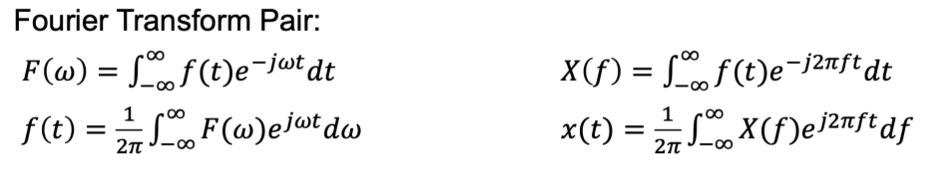
\includegraphics[width=0.99\textwidth]{figs/FT_pair.png}


	The basis functions are the complex exponentials.

	Note that both $F(\omega)$ and $f(t)$ are continuous functions and can be either 	real or complex (as with $I$ and $Q$ voltages).

	From Eulier’s Identity, we can represent cosines and sines with complex
	exponentials.

	Negative frequencies represent clockwise (CW) rotation on complex plane

	Positive frequencies represent counter-clockwise (CCW) rotation on
	complex plane 11


	Refer to ASEN5245\_Intro\_Matched\_Filter\_Compression\_013024.pdf for 		examples and further explanation.



	\item Pulse Compression Ratio [TODO]
	
	\item Decoding Phase Modulation [TODO]


\end{enumerate}

\section*{EM Basics}

\begin{enumerate}

	\item Electrostatics
	
	\begin{itemize}
	
		\item Ohms Law: $V = RI$
	
		where:
		
		V = Voltage [V]
		
		R = Resistance [$\Omega$]
		
		I = Current [Ampere]
		
		\item Electric Field
		
		$\vec{E} = \rho \vec{J}$
		
		where: 
		
		$\vec{E}$ = electric field [V/m]
		
		$\vec{J}$ = current density [A/$m^2$]
		
		$\rho$ = resistivity of the medium [$\Omega$/m]
		
		$\sigma = 1/\rho$ = conductivity 
		
		
		
		\item Coulomb's Law: $\vec{E} =  \frac{q}{4\pi \epsilon_0 r^2}\vec{R} [V/m^2]$

		where:

		$\epsilon_0$ = Permittivity of Free Space  = $\frac{1}{36\pi}*1-^{-9}$ [Farads/m]

		Dielectric Constant = $\epsilon = \epsilon_r \epsilon_0$
		
		$\vec{E}$ = electric field [V/m]
		
		$\vec{D}$ = Electric Flux Desnsity: $\vec{D} = \epsilon \vec{E}$
		
		

		$r$ = Distance between the centers of the two charges [m]
		
		\end{itemize}
		
	\item Magnetostatics
		\begin{itemize}

		\item Biot-Savart Law: $\vec{B} = \mu \vec{H}$

		where:

		$\vec{B}$ = Magnetic flux density [Tesla] = $\vec{B} = \frac{\mu_0 I}{2\pi r}$
		
		$\vec{H}$ = Magnetic field intensity [A/m]

		$\mu_0$ = Permeability of free space \(\approx 4\pi \times 10^{-7} \, \text{T m/A}\)
		$\mu = \mu_r \mu_0$ and $\mu_r = 1$ for this class
		$I$ = Electric current [A] = $\frac{dq}{dt}$

		$\vec{r}$ = Position vector from the length element to the point of observation [m]
		\end{itemize}
		
	
		
	\item Electromagnetics
		
		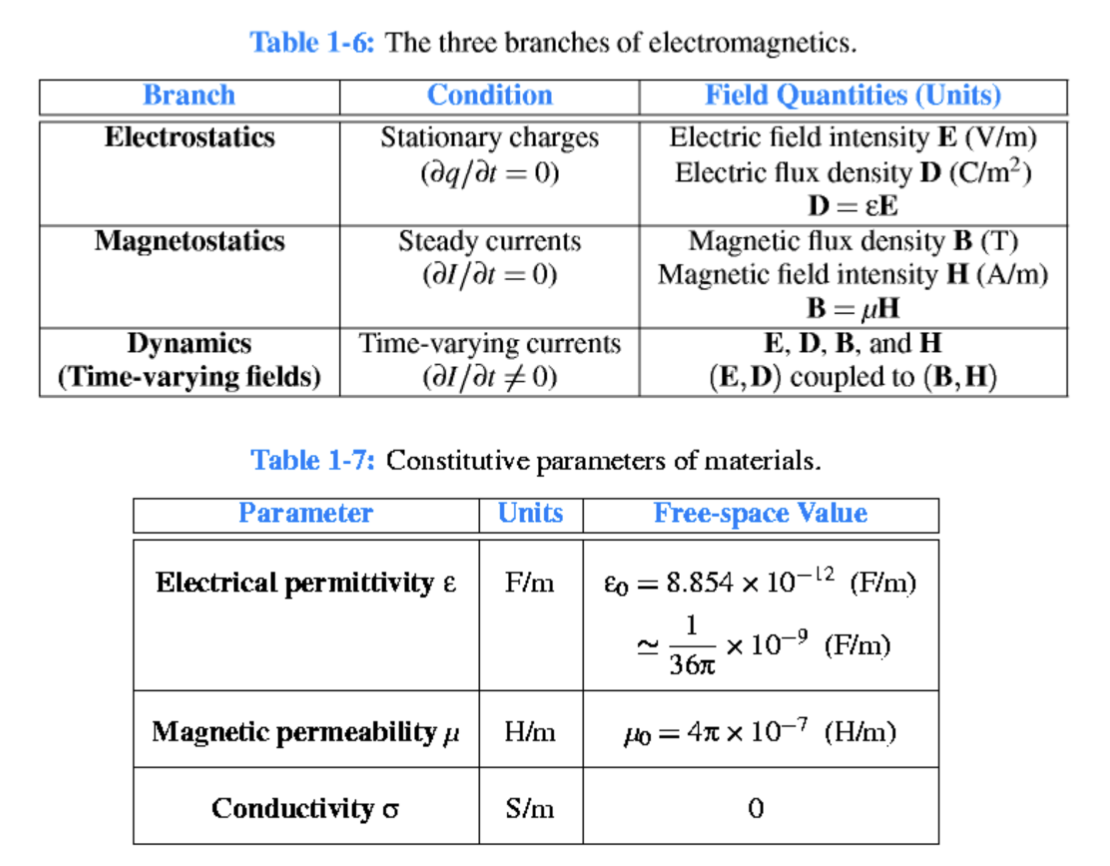
\includegraphics[width=0.99\textwidth]{figs/Electromagnetics.png}
	
	\item Maxwell’s Equations
	
	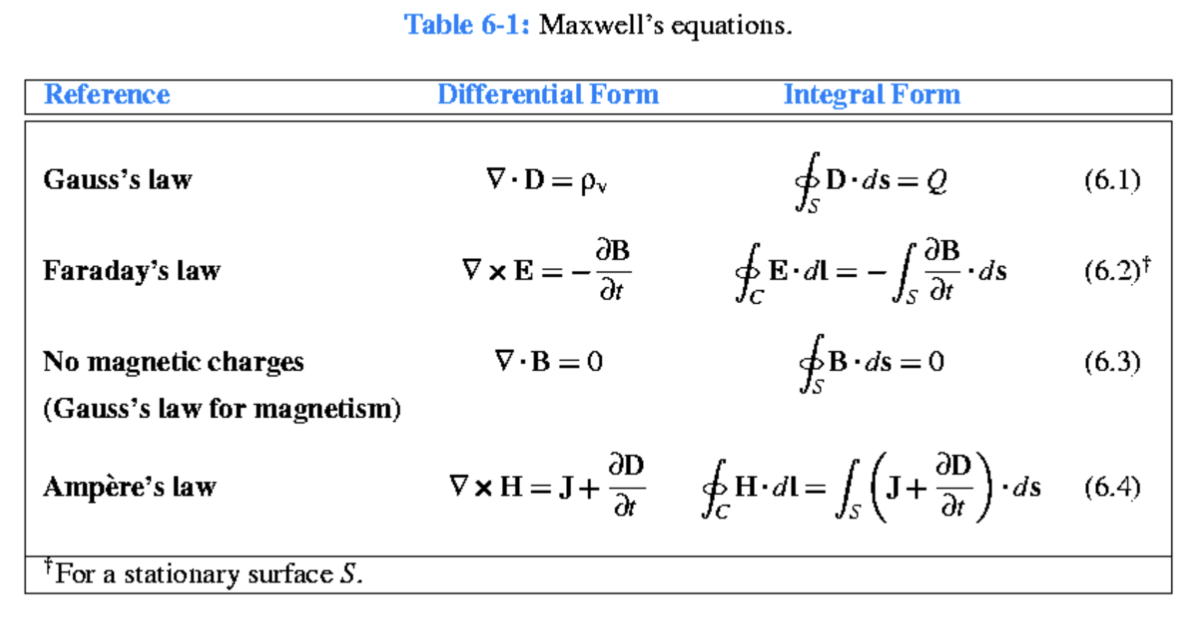
\includegraphics[width=0.99\textwidth]{figs/MaxwellsEquations.png}
	
	
	\item Phasor notation
	
	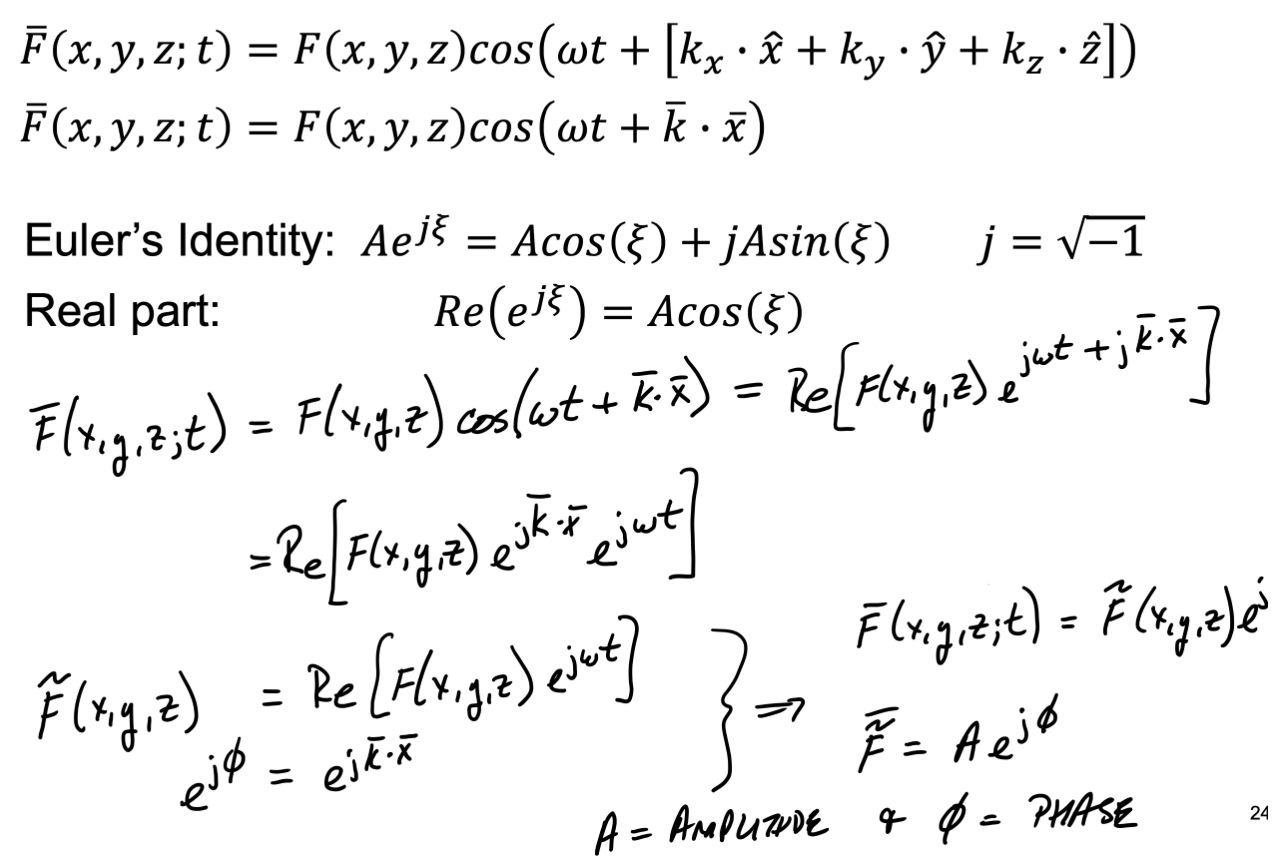
\includegraphics[width=0.99\textwidth]{figs/PhasorNotation.png}
	
	
	\item Complex permittivity
	
	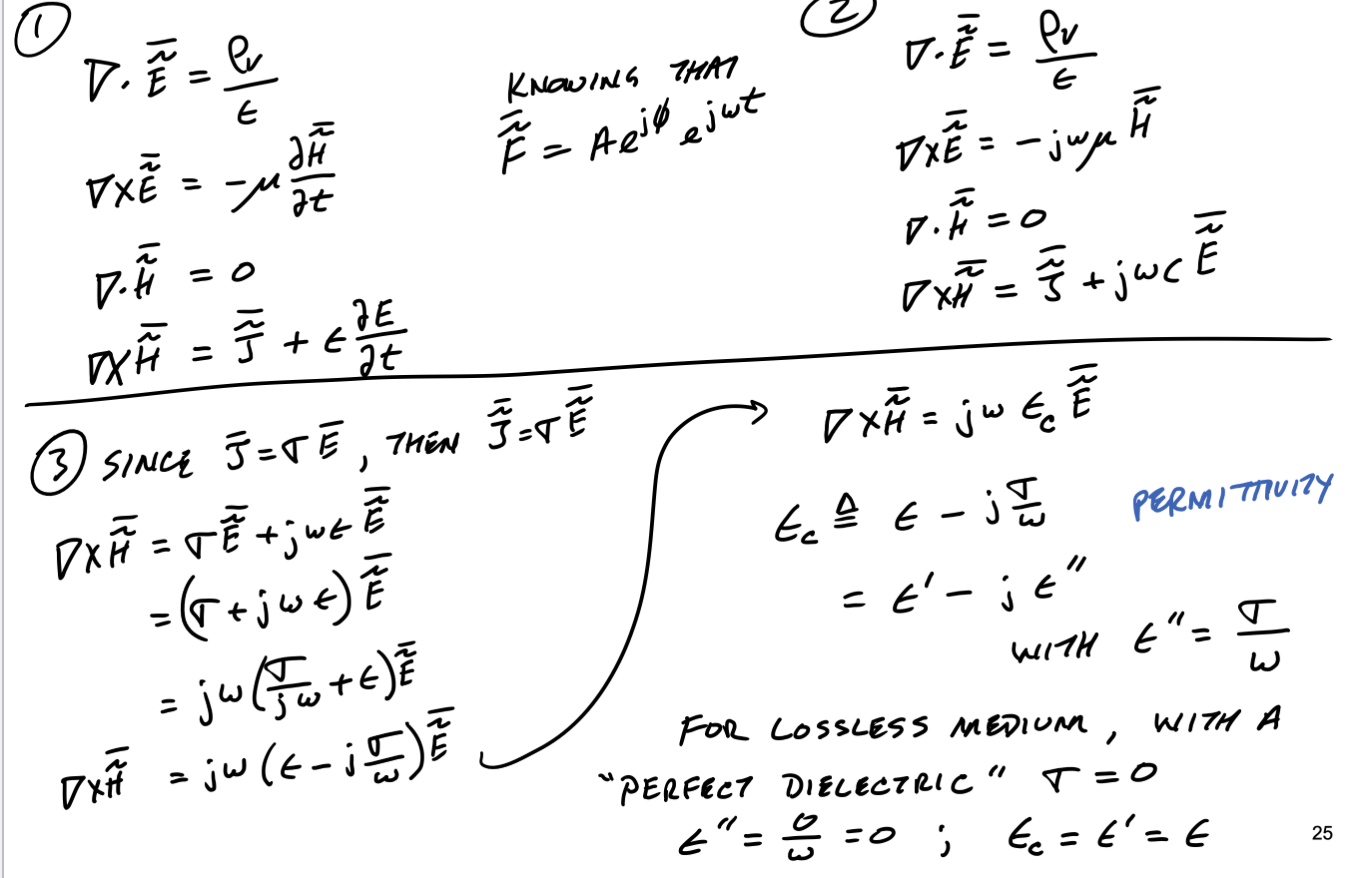
\includegraphics[width=0.99\textwidth]{figs/ComplexPermittivity.png}
	
	\item Propagating Waves
	
	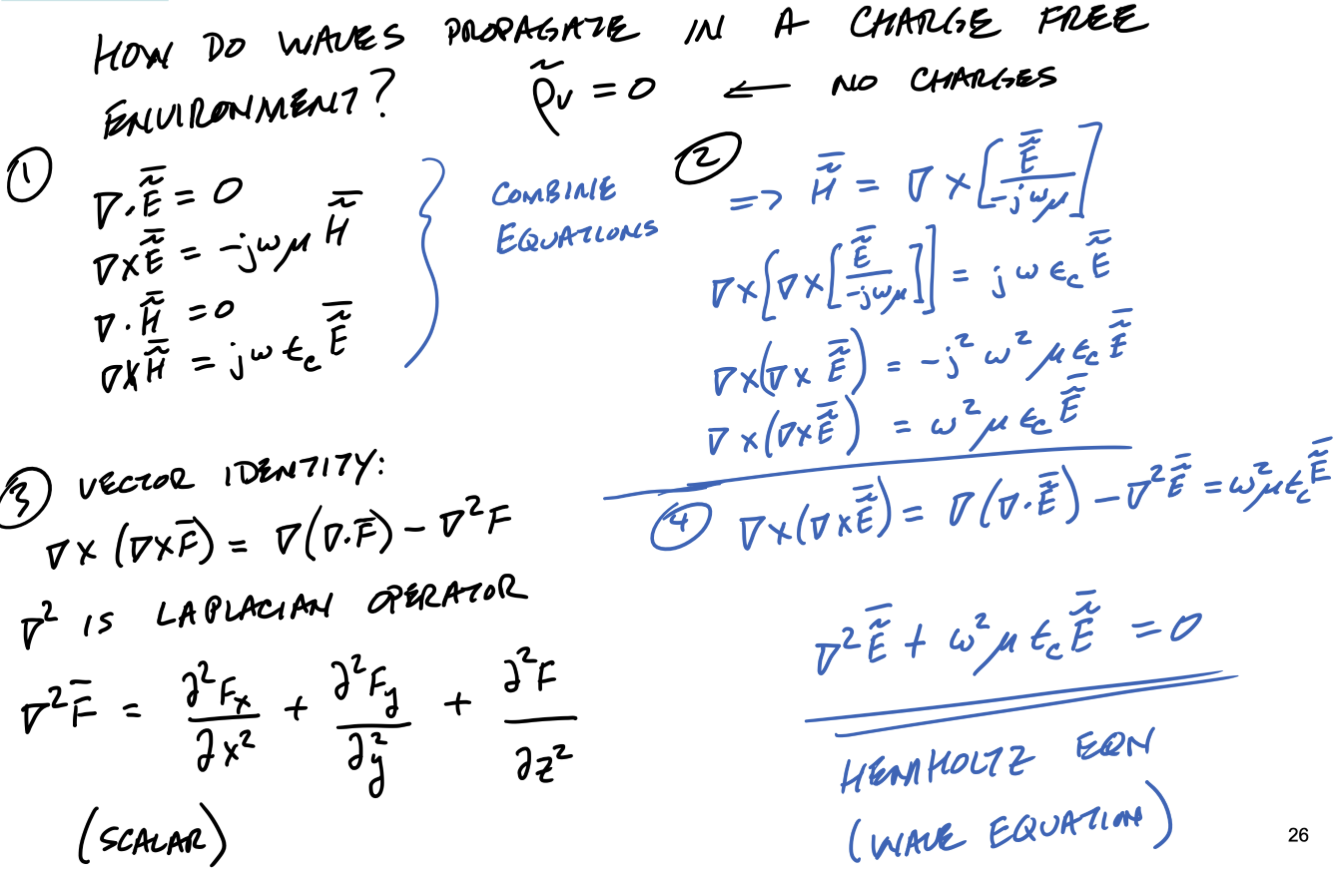
\includegraphics[width=0.99\textwidth]{figs/PropagatingWaves.png}


\end{enumerate}


\section*{Wave Propagation and Scattering}

\begin{enumerate}

	\item


\end{enumerate}


\subsection*{Antenna Properties}

\begin{enumerate}

	\item


\end{enumerate}


\subsection*{Scattering}
























\end{document}
